\documentclass{BeamerTemplate}
\title{Module 1 - Introduction aux probabilités}
\subtitle{STT-1000 Probabilités et statistique}
\date{\today}

\begin{document}
\begin{frame}[t]
  \titlepage
\end{frame}

\section{Importance de la statistique}

\begin{frame}{Importance de la statistique}
    \begin{Boite}{Pourquoi un cours de statistique}
    Conception ou analyse de systèmes ou phénomènes aléatoires, i.e. non déterministes.
    \end{Boite}
            Exemples :
        \begin{itemize}
            \item fiabilité d’une machine;
            \item quantité de pluie reçue dans un bassin versant;
            \item  demande en électricité d’un grand complexe de serveurs;
            \item nombre de tomates produites par un plant.
        \end{itemize}
\end{frame}

\begin{frame}{Probabilités vs. statistique?}
    \begin{Boite}{Probabilités}
        Outil mathématique formel servant à décrire et modéliser les comportements aléatoires.
    \end{Boite}
    On connaît les "paramètres" du phénomène et on tente de décrire ce qu'on attend du phénomène en question.


    Exemple: on lance un dé équilibré à 6 faces et on veut savoir la probabilité d'oBoitenir un «3».
    \end{frame}
    \begin{frame}{Probabilités vs. statistique?}
\begin{Boite}{Statistique}
Étude quantitative des attributs d’une “population” à partir d’observations.
    \end{Boite}
On ne connaît pas les "paramètres" du phénomène, c'est ce qu'on tente d'estimer.

Exemple: on veut savoir si un dé est équilibré...
\end{frame}

    \begin{frame}{Probabilités vs. statistique?}
Une bonne compréhenstion des probabilités et de la statistique est indispensable à la prise de décision en présence d’incertitude.
\end{frame}

\section{Expérience aléatoire}

\begin{frame}{Expérience aléatoire}
\begin{Boite}{Expérience aléatoire $\mathcal{E}$}
    Expérience dont le résultat dépend du hasard, ne pouvant être
prédit avec certitude.
\end{Boite}

\begin{Boite}{Espace échantillonnal $\mathcal{U}$}
    Ensemble de tous les résultats possibles de l’expérience $\mathcal{E}$.
\end{Boite}

\begin{itemize}
\item $\mathcal{U}$ discret : Si $\mathcal{U}$ est fini ou dénombrable \\
(ex : la liste des entiers)
\item $\mathcal{U}$ continu : Si $\mathcal{U}$ est non dénombrable\\
(ex : un intervalle de valeurs sur la droite réelle)
\end{itemize}

\end{frame}


\begin{frame}{Expérience aléatoire}
Quel est l'espace échantillonnal?

\begin{itemize}
    \item $\mathcal{E}_1$: on lance un dé et on note le chiffre sur le dessus;
    \vspace{1cm}
    \item $\mathcal{E}_2$: on pige une carte parmi les quatre rois d’un jeu standard;
    \vspace{1cm}
    \item $\mathcal{E}_3$: on compte le nombre de véhicules traversant un pont durant une heure;
    \vspace{1cm}
    \item $\mathcal{E}_4$: on mesure la quantité de pluie (en mm) reçue à une station météo au cours de l’automne.
    \vspace{1cm}
\end{itemize}
\end{frame}
\begin{frame}{Expérience aléatoire}
\begin{Boite}{Événement}
    Sous-ensemble de l’espace échantillonnal $\mathcal{U}$. On utilise une lettre majuscule pour l’identifier.
\end{Boite}
Retour aux expériences précédentes:
\begin{itemize}
    \item $\mathcal{E}_1$: $A=$“Le dé affiche un nombre pair”$=\{2,4,6\}$
     \item ${\cal{E}}_2$: \alert{$N$}=``On pige un roi noir''=$\{R\spadesuit,R\clubsuit\}$
    \item $\mathcal{E}_3$: $C=$“Moins de 100 véhicules traversent le pont”$ =\{0,1,2,...,99\}$
    \item $\mathcal{E}_4$: $D=$“La station reçoit plus de 150 mm de pluie”$=(150,\infty)$
\end{itemize}

\end{frame}


\begin{frame}{Expérience aléatoire}
\begin{tabular}{lll}
1) Complément de $A$: $\overline{A}$&\hspace{1cm}&2) Inclusion de $B$ dans $A$: $B \subset A $\\
&&\\
\begin{tabular}{|ccc|}\hline
&&\\[-0.2cm]
\hspace{0.05cm}&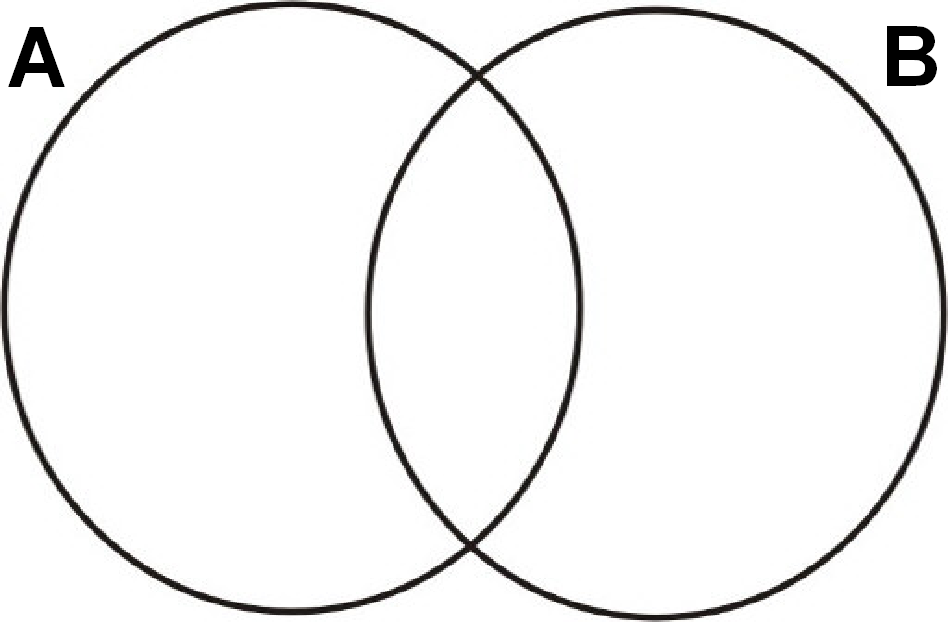
\includegraphics[width=2.7cm]{venn.pdf}&\hspace{.05cm}\\
\hline
\end{tabular}&&
\begin{tabular}{|ccc|}\hline
&&\\[-0.2cm]
\hspace{0.05cm}& \hspace{2.7cm} &\hspace{.05cm}\\[1cm]&&\\
\hline
\end{tabular}\\

&&\\
%&&\\
3) Intersection de $A$ et $B$: $A\cap B$&\hspace{1cm}& 4) Union de $A$ et $B$: $A\cup B$\\&&\\%&&\\
\begin{tabular}{|ccc|}\hline
&&\\[-0.2cm]
\hspace{0.05cm}&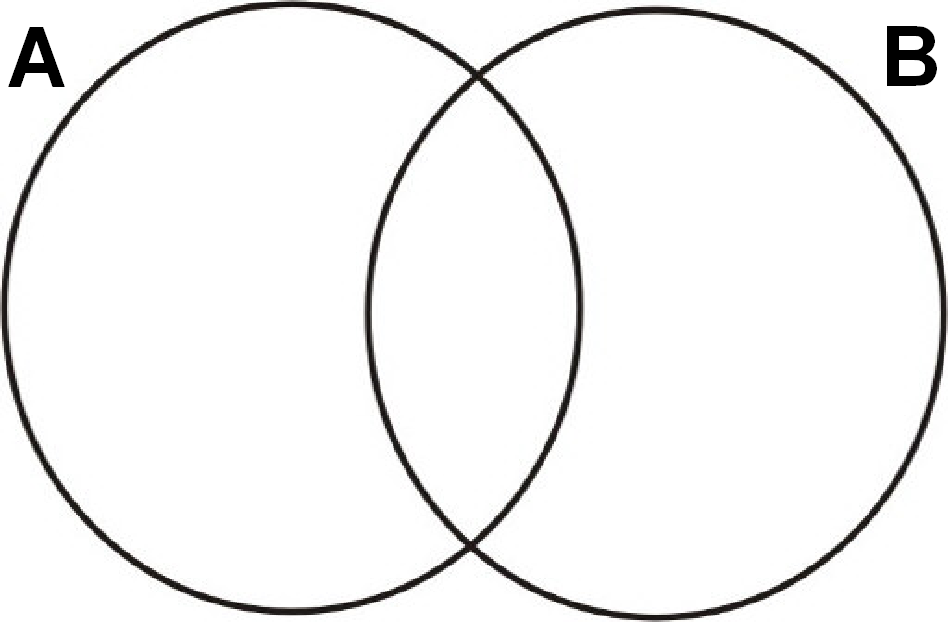
\includegraphics[width=2.7cm]{venn.pdf}&\hspace{.05cm}\\
\hline
\end{tabular}
&\hspace{1cm}&
\begin{tabular}{|ccc|}\hline
&&\\[-0.2cm]
\hspace{0.05cm}&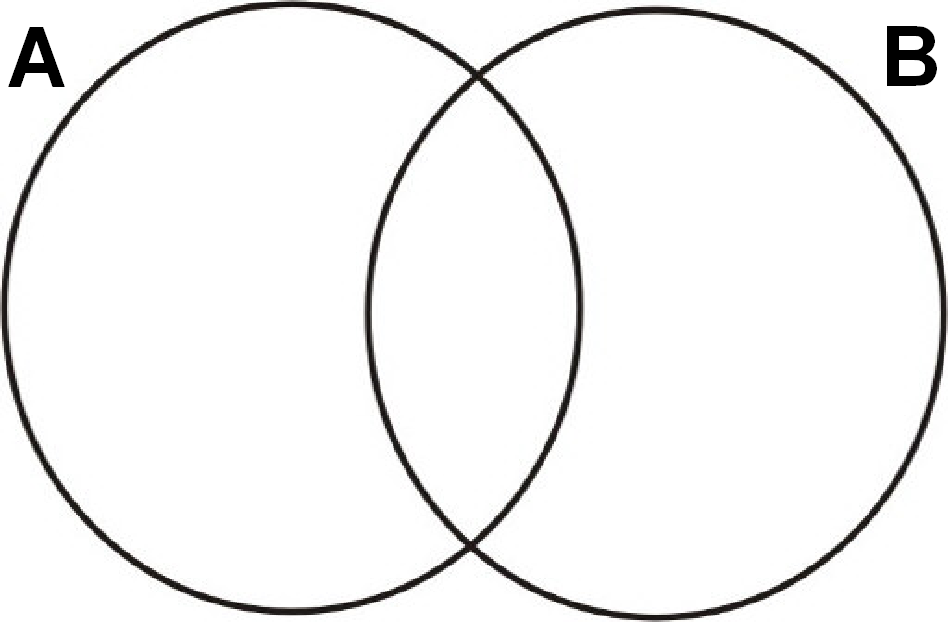
\includegraphics[width=2.7cm]{venn.pdf}&\hspace{.05cm}\\
\hline
\end{tabular}
\end{tabular}

\vspace{1cm}
\end{frame}

\begin{frame}[t]{Expérience aléatoire}
    Autres éléments importants
\begin{itemize}
    \item L'\alerter{ensemble vide} est l'ensemble qui ne contient aucun élément. Dénoté $\emptyset$
    \item $\emptyset$ est inclus dans tout ensemble $A$\\
    $\emptyset \subset A, \forall A$
    \item Tout ensemble $A$ est inclus dans $\mathcal{U}$\\
    $A\subset \mathcal{U}, \forall A$
    \item Deux ensembles $A$ et $B$ sont \alerter{égaux} si, et seulement si, $A$ est un sous-ensemble de $B$ et $B$ est un sous-ensemble de $A$.\\
    $A=B \iff A\subset B$ et $B\subset A$
    \item $A\subset B$ et $B\subset C$ implique $A\subset C$
    \item L'ordre des éléments dans un ensemble n'a pas d'importance\\
    $A=\{1,2,3,4,5,6\}$ est le même ensemble que $A=\{6,5,4,3,2,1\}$
\end{itemize}
\end{frame}

\begin{frame}[t]{Expérience aléatoire}
\scriptsize{
    Lois d'identités
    \begin{align*}
        A\cup \emptyset = A & & A\cup \mathcal{U} = \mathcal{U}\\
        A\cap \emptyset = \emptyset & & A\cap \mathcal{U} = A
    \end{align*}
    Lois de De Morgan
    \begin{align*}
        \overline{A\cup B}&=\overline{A}\cap \overline{B}\\
        \overline{A\cap B}&=\overline{A}\cup \overline{B}\\
    \end{align*}
    Lois associatives
    \begin{align*}
        A\cup (B\cup C) &= (A\cup B)\cup C\\
        A\cap (B\cap C) &= (A\cap B)\cap C
    \end{align*}
    Lois distributives
        \begin{align*}
        A\cup (B\cap C) &= (A\cup B)\cap (A \cup C)\\
        A\cap (B\cup C) &= (A\cap B)\cup (A \cap C)\\
    \end{align*}
    }
\end{frame}

\begin{frame}{Expérience aléatoire}
 \begin{Boite}{Événements mutuellement exclusifs}
  Des événements sont \alert{mutuellement exclusifs} si toutes
  leurs combinaisons possibles d'intersections sont vides, c'est-à-dire
  lorsqu'\textbf{au plus un} de ces événements peut se produire à
  la fois. 
 \end{Boite}

 \medskip

\pause


 En d'autres termes, $A$, $B$ et $C$ sont mutuellement exclusifs, si

  \begin{itemize}
   \item $A\cap B=\emptyset$
   \item $A\cap C=\emptyset$
   \item $B\cap C=\emptyset$
   \item $A\cap B\cap C=\emptyset$
 \end{itemize}

\end{frame}

\begin{frame}[t]%{Événements mutuellement exclusifs}

\centerline{\LARGE \bf \alert{QUIZ !}}
 Les événements suivants sont-ils mutuellement exclusifs?
 \medskip

 {\small  %Retour aux exemples:
  \begin{itemize}\itemsep1.3cm
   \item $\mathcal{E}_1$: Lancer d'un dé.\\
   Soient $A=$``oBoitenir un nombre pair'', $B=\{5\}$ et $C=\{1\}$. \\
   %Comme    $A\cap B=A\cap C=B\cap C=A\cap B\cap C=\emptyset$, ces trois    événements sont mutuellement exclusifs.
   \item $\mathcal{E}_4$: Mesurer les précipitations.\\
   $A=$``La station re\c{c}oit plus de 150 mm'',\\
   $B=$``La station re\c{c}oit moins de 175 mm'' et \\$C=$``La station re\c{c}oit
   entre 200 et 300 mm''. \\%Comme $A\cap B=(150,175)\neq\emptyset$,     $A,B,C$ ne sont \alert{pas} mutuellement exclusifs. (Même si $B$ et $C$ le sont.)
   %(On aurait aussi pu    utiliser $A\cap C=(300,\infty)\neq\emptyset\ldots$)
   \vspace{1.3cm}
 \end{itemize}
 }
\end{frame}


\section{Probabilités}

\subsection{Définitions et notation}

\begin{frame}[t]%{Définition mathématique}

\begin{defn}{}
  Soit une expérience aléatoire $\mathcal{E}$ et son espace échantillonnal
  $\mathcal{U}$. \\Si un événement $A$ est défini dans $\mathcal{U}$, alors la \alerter{probabilité
  de $A$, notée $P(A)$}, est un nombre réel respectant les axiomes
  suivants:
  \begin{enumerate}
   \item $0\le P(A)\le 1$
   \item $P(\mathcal{U})=1$
   \item Pour toute suite d'événements \alerter{mutuellement exclusifs}
   $A_1,A_2,\ldots,A_k$ définis dans $\mathcal{U}$, on a
   $$P(A_1\cup A_2\cup \cdots \cup A_k)=P(A_1)+P(A_2)+\cdots+P(A_k)$$
   \item L'axiome 3 reste vrai quand $k\to\infty$ :\ $P\left(\bigcup_{i=1}\limits^\infty A_i\right)=\sum\limits_{i=1}^\infty P(A_i)$.
  \end{enumerate}
 \end{defn}

\end{frame}

\begin{frame}[t]{Spécification des probabilités}
Comment peut-on déterminer des probabilités?
\medskip

 \begin{itemize}\itemsep8mm
  \item<1-> estimations basées sur des observations
  \item<2-> analyse des conditions expérimentales
  \item<3-> modèles probabilistes et/ou hypothèses
 \end{itemize}
\end{frame}

\subsection{Propriétés}

\begin{frame}[t]{Résultats découlant des axiomes}
Les résultats qui suivent sont des conséquences des 4 axiomes
définissant une probabilité.
 \begin{itemize}
  \item<1->{\bf Théorème 1.1}: $P(\emptyset)=0$

  {\color{gray}{[$\mathcal{U}$ et $\emptyset$ sont mutuellement
  exclusifs, $\mathcal{U}\cup\emptyset=\mathcal{U}$ et $P(\mathcal{U})=1$ ...]}}
  \item<2->{\bf Théorème 1.2}: $P(\bar{A})=1-P(A)$

  {\color{gray}{[$A$ et $\bar{A}$ sont mutuellement
  exclusifs et $\mathcal{U}=A\cup\bar{A}$ ...]}}
  \item<3->{\bf Théorème 1.3}: $P(A\cup B)=P(A)+P(B)-P(A\cap B)$

  \item<4->{\bf Théorème 1.4}:
  $$\begin{array}{lll}
  P(A\cup B\cup C)&=&P(A)+P(B)+P(C)\\&&-P(A\cap B)
   -P(A\cap C)-P(B\cap C)\\&&+P(A\cap B\cap C)\end{array}$$

 \end{itemize}
\end{frame}

\begin{frame}[t]{Résultats découlant des axiomes (suite)}
 \begin{itemize}\itemsep6mm
  \item<1->{\bf Théorème 1.5}: Généralisation de 1.4 à $k$ événements:
     \\
$P\left(\bigcup\limits_{i=1}^kA_i\right)=\sum\limits_{i=1}^kP(A_i)
  -\sum\limits_{i=1}^k\sum\limits_{j=i+1}^kP(A_i\cap A_j)+\cdots+(-1)^{k-1}P\left(\bigcap\limits_{i=1}^kA_i\right)$

  \item<2->{\bf Théorème 1.6}: Si $A\subset B$, alors $P(A)\le P(B)$.

  {\small \color{gray}{[$B=(\bar{A}\cap B)\cup A$, et $(\bar{A}\cap B)$ et $A$ sont mutuellement exclusifs ...]}}
 \end{itemize}
\end{frame}

\begin{frame}[t]%{Événements mutuellement exclusifs}

\centerline{\LARGE \bf \alert{QUIZ !}}
\begin{minipage}{8cm}{
\small
Vous achetez un nouveau téléphone. \\
D\'efinissons les \'ev\'enements suivants:\\
$A$: La carte SIM est d\'efectueuse.\\
$B$: La batterie a une autonomie insuffisante.\\
}
\end{minipage}

\vspace{.3cm}

Chez ce fournisseur, $P(A)=0,05$, $P(B)=0,20$ et $P(A \cup B)=0,23$.

\begin{enumerate}[{a)}]\itemsep1cm
  \item Quelle est la probabilité que votre batterie dure suffisamment longtemps?
  \item Quelle est la probabilité que les deux problèmes soient présents sur le téléphone que vous avez acheté?
\end{enumerate}
\end{frame}



\begin{frame}[t]{Exemple 2 suite}
Dans l'exemple précédent, quelle est la probabilité qu'aucun des deux problèmes n'affecte votre téléphone?

 \bigskip

 (Indice: Tracez le diagramme de Venn de ces ensembles en inscrivant les probabilités dans les régions représentées.)

 \bigskip
Rappel:   $P(A)=0,05$, $P(B)=0,20$ et $P(A \cup B)=0,23$.
\vspace{3cm}

\end{frame}

\begin{frame}[t]{Exemple 3}

\begin{minipage}{8cm}{
\small
 \`A l'Université ABC,
 \begin{enumerate}[$\bullet$]
 \item 55\% des étudiants portent des lunettes,
 \item 70\% des étudiants possèdent un portable,
 \item 75\% des étudiants sont satisfaits de leurs études.
 \end{enumerate}
 }
 \end{minipage}


 \bigskip
 {\small
 Si on choisit un étudiant au hasard dans cette université, pouvez-vous déterminer la probabilité qu'il s'agisse...
  \begin{enumerate}[(i)]\itemsep.8cm
 \item d'un étudiant qui ne porte pas de lunettes? % 0.45
  \item d'un étudiant avec lunettes satisfait de ses études? % infos insuffisantes
 \end{enumerate}
}
\end{frame}

\begin{frame}[t]{Exemple 3 (suite)}

{\footnotesize
 On vous informe également qu'à l'Université ABC,
 \begin{enumerate}[$\bullet$]
 \item 35\%  des étudiants portent des lunettes et possèdent un portable,
 \item 30\% portent des lunettes, sont satisfaits de leurs études et possèdent un portable,
 \item 5\% portent des lunettes, sont insatisfaits de leurs études et n'ont pas de portable,
%  \item 13\% sont des gar\c{c}ons  satisfaits de leurs études.
 \end{enumerate}
 Pouvez-vous maintenant déterminer la probabilité qu'un étudiant choisi au hasard soit...
     \begin{enumerate}\itemsep 4mm
      \item[(iii)] un étudiant avec lunettes, satisfait de ses études?% 0.45
      \item[(iv)] sans lunettes et  satisfait de ses études? %0.30
      \item[(v)] sans lunettes et satisfait de ses études et possédant un portable? % infos insuffisantes
      \item[(vi)] une personne satisfaite ou ayant des lunettes?% 0.85
     \end{enumerate}
}
\end{frame}

\begin{frame}[t]{Exemple 3: piste de solution}

{\small
 Remplir toutes les zones mutuellement exclusives d'un diagramme de Venn.\\
 $L=$``l'étudiant porte des lunettes'', $P=$``l'étudiant possède un
 portable'' et $S=$``l'étudiant est satisfait de ses études''. %On cherche (i) $P(\bar{F}\cap P\cap \bar{S})$ et (ii) $P(F\cap \bar{P}\cap S)$.
}

\centerline{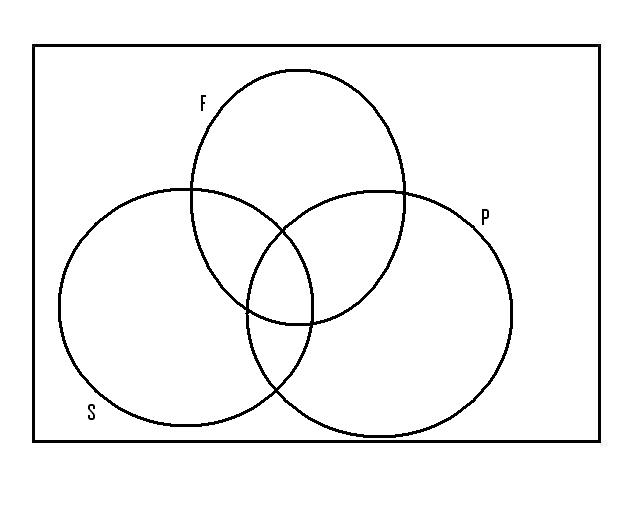
\includegraphics[height=5cm]{venn-eg.jpg}}
\end{frame}
\begin{frame}[t]{Exemple 3: des infos partielles}
\begin{enumerate}
\item[(vii)] Si on vous disait que l'étudiant pigé est satisfait de ses études, pourriez-vous déterminer la probabilité qu'il porte des lunettes?

\vspace{1.3cm}

\item[(viii)] Sauriez-vous déduire de vos informations la probabilité qu'un étudiant avec lunettes choisi au hasard possède un portable?

\vspace{1.3cm}
\end{enumerate}

Pour faire ces calculs, vous devez utiliser une information partielle, qui réduit l'espace échantillonnal. Vous calculerez des {\it probabilités conditionnelles}...

\end{frame}

\section{Probabilités conditionnelles}



\begin{frame}[t]%{Probabilité conditionnelle}
 \begin{Boite}{Probabilité conditionnelle}
  Soient $A$ et $B$ deux événements dans $\mathcal{U}$ avec $P(B)>0$. Alors
  la \alert{probabilité conditionnelle} de $A$  sachant que  $B$ s'est réalisé est
  $$P(A|B)=\frac{P(A\cap B)}{P(B)}.$$
 \end{Boite}
\end{frame}

\begin{frame}[t]{Propriétés}
 Une probabilité conditionnelle a toutes les propriétés d'une probabilité:

 \begin{enumerate}\itemsep3mm
  \item $0\le P(A|B)\le 1$
  \item $P(\mathcal{U}|B)=P(B|B)=1$
  \item Soit $A_1,\ldots,A_k$ une suite d'événements \textcolor{red}{mutuellement
  exclusifs}. Alors $P\left(\left.\bigcup\limits_{i=1}^kA_i\right|B\right)=\sum\limits_{i=1}^k P(A_i|B)$.
  \item La propriété 3 demeure vraie quand $k\to\infty$.
 \end{enumerate}
\end{frame}

\begin{frame}[t]{Règle de multiplication}
On peut utiliser la définition de probabilité conditionnelle pour déduire la valeur de $P(A\cap B)$:
$$P(A|B)=\frac{P(A\cap B)}{P(B)}\quad\Leftrightarrow\quad P(A\cap B)=P(A|B)P(B).$$
On appelle parfois cette formule ``règle de multiplication''.
\end{frame}
\begin{frame}[t]{Exemple 4}

{\small
 \begin{enumerate}[$\bullet$]\itemsep3mm
 \item 70\% des pièces électroniques que vous utilisez viennent de l'usine A et les autres pièces viennent de l'usine B.
 \item 25\% de toutes les pièces sont défectueuses.
 \item 10\% de toutes les pièces viennent de l'usine A et sont défectueuses.
 \item[a)] On vous donne une  pièce qui vient de l'usine A. Quelle est la probabilité qu'elle soit défectueuse?
\item[b)] On vous donne une pièce défectueuse. Quelle est la probabilité qu'elle proviennent de l'usine B?
     \end{enumerate}
     }
\end{frame}

\begin{frame}[t]%{Événements mutuellement exclusifs}

\centerline{\LARGE \bf \alert{QUIZ !}}
Supposons $P(B)>0$.
\vspace{3mm}

\begin{itemize}\itemsep1.5cm
\item Que vaut $P(A|B)$ si $B\subset A$?

\item Que vaut $P(A|B)$ si $A\subset B$?

\item Que vaut $P(A|B)$ si $A$ et $B$ sont mutuellement exclusifs?
\vspace{1cm}
\end{itemize}
\end{frame}

\subsection{Indépendance}

\begin{frame}[t]{Indépendance de deux événements}
 %Dans plusieurs situations, le fait que l'événement $B$  se réalise n'a aucun effet sur la probabilité que l'événement  $A$ se produise.

 \bigskip
 Je roule un dé, puis je lance une pièce  de monnaie. \\Soit les événements\\
  $A=$``le dé indique 6'', et \\
  $B=$``la pièce indique  face''. \\

  \bigskip

Le fait que $A$ se réalise ou non n'a aucun impact sur la probabilité d'oBoitenir pile ou face!
\bigskip

On dira alors que $A$ et $B$ sont \textcolor{red}{indépendants}. Voyons une définition plus mathématique de l'indépendance d'événements.
\end{frame}


\begin{comment}
{\small
 \begin{block}{Théorème 1.7}
  \begin{itemize}
   \item<1-> $A\perp B\Leftrightarrow A\perp \bar{B}$
   \item<1-> $A\perp B\Leftrightarrow \bar{A}\perp \bar{B}$
   \item<1-> $A\perp B\Leftrightarrow \bar{A}\perp {B}$
  \end{itemize}
 \end{block}

 \medskip
 \uncover<2->{
  \begin{block}{Impact sur les probabilités conditionnelles}
   Supposons que $P(B)>0$, de sorte que $P(A|B)$ est bien définie.
   \begin{itemize}
    \item Si $A\perp B$, alors $P(A|B)=P(A)$.
    \item Si $P(A)>0$ aussi, alors $P(A|B)=P(A)\Leftrightarrow A\perp B$.
   \end{itemize}
  \end{block}
  }}
  \end{comment}

\begin{frame}[t]%{Indépendance de deux événements}
 \begin{Boite}{Indépendance de deux événements}
  Soient $A$ et $B$ deux événements de $\mathcal{U}$. On dit que $A$ et $B$
  sont \alert{indépendants, noté $A\perp B$}, si et seulement si
  $$P(A\cap B) = P(A)P(B).$$
 \end{Boite}

    \begin{Boite}{Impact sur les probabilités conditionnelles}
   Supposons que $P(B)>0$, de sorte que $P(A|B)$ est bien définie.\\
   \alert{Si $A$ et $B$ sont indépendants}, alors
   $$P(A|B)=P(A)$$
   À l'inverse, si cette condition est remplie, alors $A$ et $B$ sont indépendants.
  \end{Boite}
\end{frame}

\begin{frame}[t]{Questions}
 \begin{enumerate}\itemsep 2cm
 \item   Des événements mutuellement exclusifs sont-ils  indépendants en général?
 \item Si $A\subset B$, a-t-on que $A$ et $B$ sont indépendants, en général?
\end{enumerate}
\end{frame}

\begin{frame}[t]{Généralisation à $k$ événements}
 \begin{defn}{}
  On dit de $k$ événements qu'ils sont \textcolor{red}{mutuellement
  indépendants} si, et seulement si, les probabilités de
  \textcolor{red}{toutes} les intersections de $2,3,\ldots,k$ d'entre
  eux sont égales aux produits de leurs probabilités
  respectives.
 \end{defn}

 \medskip
 Par exemple, $A,B,C$ sont indépendants si et seulement si \\
 $P(A\cap B)=P(A)P(B)$ ET \\
 $P(A\cap C)=P(A)P(C)$ ET \\
 $P(B\cap C)=P(B)P(C)$ ET \\
 $P(A\cap B\cap C)=P(A)P(B)P(C)$.
\end{frame}

\begin{frame}[t]{Exemple 5}

$A$ et $B$ sont-ils indépendants?

 \centerline{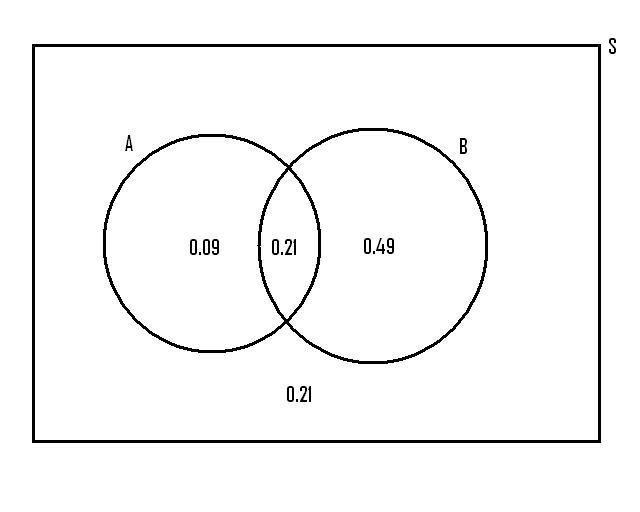
\includegraphics[height=5cm]{venn1-p22.jpg}}

\end{frame}

\begin{frame}[t]{Exemple 6}

Il est possible que $A\perp B$, $A\perp C$ et $B\perp C$, mais
que $A,B,C$ ne
soient pas indépendants. Par exemple

 \centerline{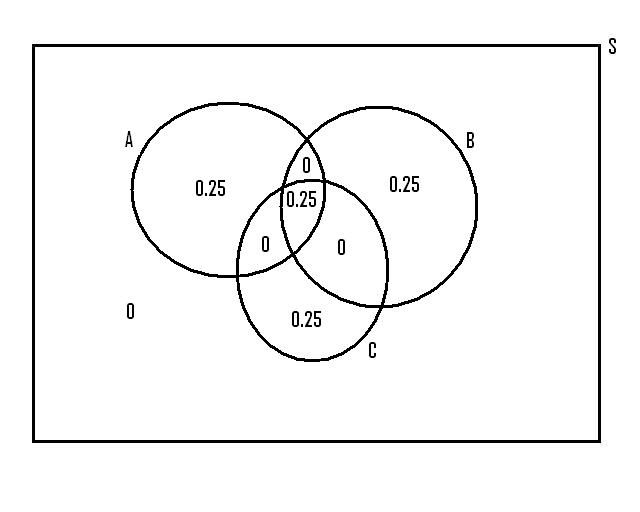
\includegraphics[height=5cm]{venn2-p22.jpg}}

\end{frame}

%\section{Loi des probabilités totales, théorème de Bayes}

\subsection{Loi des probabilités totales}

\begin{frame}[t]{Partitionner l'espace échantillonal}

{\small Plusieurs problèmes de calcul de probabilités
 deviennent plus simples si on les divise en
 plusieurs morceaux. %\`A cette fin, nous voudrons  \alert{partitionner} l'espace échantillonnal.

 \begin{Boite}{Partition de l'espace échantillonnal}
  On dit que $B_1,B_2,\ldots,B_k$ forment une \alert{partition
  de $\mathcal{U}$} si et seulement si
  \begin{enumerate}
   \item ils sont mutuellement exclusifs, i.e., $B_i\cap B_j=\emptyset,\ \forall i\neq j$\\

   \underline{et}
   \item leur union est $\mathcal{U}$: $B_1\cup B_2\cup ...\cup B_k=\mathcal{U}$.
  \end{enumerate}
 \end{Boite}
}
\end{frame}

\begin{frame}[t]{Exemple d'une partition de $\mathcal{U}$}

 \centerline{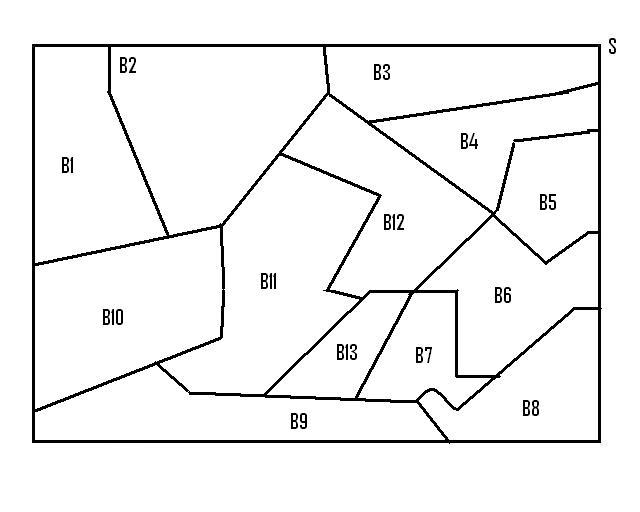
\includegraphics[height=6.8cm]{partition-p24.jpg}}

\end{frame}

\begin{frame}[t]{Utilité de partitionner $\mathcal{U}$}
 \begin{Boite}{Lemme}
  Si $B_1,\ldots,B_k$ forment une partition de $\mathcal{U}$ et
  $A$ est un événement dans $\mathcal{U}$, alors
  $$A=(A\cap B_1)\cup(A\cap B_2)\cup\cdots\cup(A\cap B_k).$$

  Puisque $(A\cap B_i)\cap(A\cap B_j)=\emptyset,\ \forall i\neq j$, on a que
  \begin{align*}
  P(A)&=P(A\cap B_1)+P(A\cap B_2)+\cdots+P(A\cap B_k)\\
  \alert {P(A)} &\alert{=\sum_{i=1}^kP(A\cap B_i)}.
  \end{align*}
 \end{Boite}
\end{frame}

\begin{frame}[t]{Exemple d'une partition de $\mathcal{U}$}

 \centerline{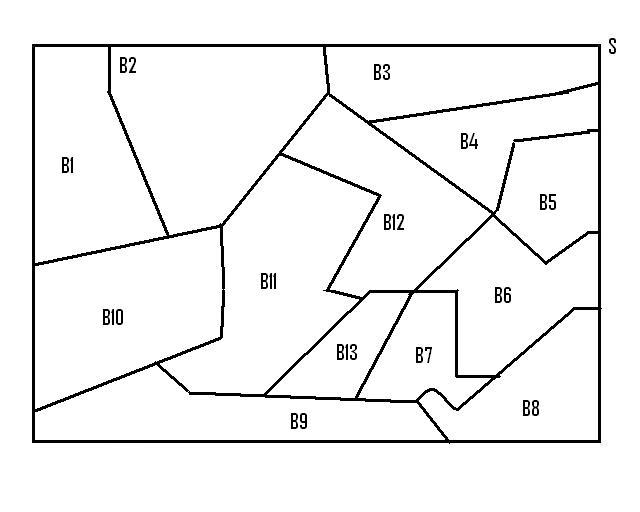
\includegraphics[height=6.8cm]{partition-p24.jpg}}

\end{frame}

\begin{frame}[t]{Conditionner sur une partition pour trouver $P(A)$}
 \begin{thm}{Loi des probabilités totales}\\
  Soit $A$ un événement dans $\mathcal{U}$ et $B_1,\ldots,B_k$ une partition
  de $\mathcal{U}$. Alors
  $$\begin{array}{llccccc}
P(A)&=& P(A\cap B_1) &+&...&+&P(A\cap B_k)\\
&&&&&&\\
    &=&P(B_1)P(A|B_1)&+&...&+&P(B_k)P(A|B_k)\\
&&&&&&\\
    &=&\multicolumn{5}{l}{\sum\limits_{i=1}^k P(B_i)P(A|B_i)}\\
\end{array}
$$
 \end{thm}


 \bigskip
 \underline{Cas particulier}: Comme $B$ et $\overline{B}$ forment une partition
 de $\mathcal{U}$, on a $P(A)=P(A|B)P(B)+P(A|\overline{B})P(\overline{B})$.
\end{frame}
\begin{frame}[t]{Exemple 7}

{\small Je suis de bonne humeur 75\% du temps. Quand je suis de bonne humeur, j'enseigne
 bien 90\% du temps. Quand je ne suis pas de bonne humeur, j'enseigne bien 20\%
 du temps.

\begin{enumerate}\itemsep 2cm
\item[a)] Quelle est la probabilité que je ne sois pas de bonne humeur et que je n'enseigne
 pas bien?
\end{enumerate}

}
\end{frame}
\begin{frame}[t]{Exemple 7 (suite)}

{\small
\begin{enumerate}\itemsep 2cm
\item[b)]  Quelle est la probabilité que j'enseigne bien?
\end{enumerate}


 \vspace{5 cm}

}
\end{frame}

\begin{frame}[t]{Exemple 8}

{\footnotesize Dans un certain pays,
\begin{enumerate}[$\bullet$]
\item 50\% des viaducs sont faits en béton de type A,
\item 30\% des viaducs sont faits en béton de type B et
\item 20\% des viaducs sont  faits avec des matériaux autres que le béton.
\end{enumerate}

On sait aussi que
\begin{enumerate}[$\circ$]
\item 90\% des viaducs faits de béton de type A vont résister sans travaux majeurs  pendant plus de 10 ans,
\item cette proportion est de 80\% chez les viaducs
 faits de béton de type B
 \item et de 70\% chez les viaducs faits en des matériaux
 autres que le béton.
\end{enumerate}

\bigskip

}
\end{frame}

\begin{frame}[t]{Exemple 8 (suite)}
Tracez un diagramme en arbre et un diagramme de Venn qui schématise cette situation.
 \vspace{7cm}
\end{frame}


\begin{frame}[t]
Exemple 8: Quelle est la probabilité qu'un viaduc pris au  hasard dans ce pays résiste plus de 10 ans sans travaux majeurs?

 \vspace{5.6cm}


\end{frame}

\subsection{Théorème de Bayes}

\begin{frame}[t]{Quand l'information est donnée ``à l'envers'' ...}
 Pour plusieurs problèmes, on donne l'information sous la forme $P(A|B_i)$,
 mais on nous demande de calculer $P(B_i|A)$.

 \begin{itemize}\itemsep 1cm
  \item Dans l'exemple de mon humeur (ex. 7), quelle est la probabilité que je sois
  de bonne humeur sachant que j'enseigne bien?
  \item Dans l'exemple des viaducs (ex. 8), si un viaduc a résisté moins de 10 ans
  sans travaux majeurs, quelle est la probabilité qu'il soit fait de béton
  de type B?
 \end{itemize}
\end{frame}

\begin{frame}
 \begin{thm}{}
  Soient $A$ un événement dans $\mathcal{U}$ et $B_1,\ldots,B_k$, une partition
  de $\mathcal{U}$. Alors
  $$P(B_j|A)=\frac{P(A|B_j)P(B_j)}{\sum_{i=1}^kP(A|B_i)P(B_i)},\ \ \forall j=1,\ldots,k.$$
 \end{thm}
On nomme ce théorème, le \textit{Théorème de Bayes}. Il s'agit d'un des résultats les plus importants de la théorie des probabilités.

\end{frame}

\begin{frame}[t]{Exemple 7 (suite)}

Imaginons que j'enseigne bien aujourd'hui(!).
\bigskip

Quelle est la probabilité que je sois de bonne humeur, sachant cette information?

\end{frame}


\begin{frame}[t]%{Événements mutuellement exclusifs}

\centerline{\LARGE \bf \alert{QUIZ !}}
  Retournons à l'exemple 8. Un pan de viaduc s'est effondré le mois passé, 8 ans après la construction. Quelle est la probabilité que ce viaduc soit fait de béton
  de type B?
 \vspace{5cm}
 

\end{frame}

\section{Permutation et combinaison}

\begin{frame}[t]{Permutation}
 \begin{defn}{}
  Une \textcolor{red}{permutation} est un arrangement \textcolor{red}{ordonné}
  d'objets \textcolor{red}{distincts}.
 \end{defn}

 \medskip

 \uncover<2->{
  \underline{Exemple}: \\
  Il reste 3 gâteaux sur la table : chocolat, vanille et café. Deux personnes souhaitent en manger un. De combien de façons
  différentes peut-on assigner les gâteaux aux 2 personnes?
 }

%On a 6 \alert{permutations} possibles  de 3 objets pris deux \`a la fois.
\end{frame}

\begin{frame}{Permutations - Formule g\'en\'erale}

 \begin{Boite}{Permutation}
  Le nombre de permutations possibles de $n$ objets pris $r$
  à la fois est donné par
  $$P_r^n=n(n-1)\cdots(n-r+1)=\frac{n!}{(n-r)!}.$$
 \end{Boite}

 \medskip

 \uncover<2->{
  Ce résultat vient du \textcolor{red}{principe de multiplication}: nous avons $n$
  choix d'objets pour la première position, $n-1$ choix d'objets pour la
  seconde position, ..., $n-r+1$ choix d'objets pour la $r$-ème position.
 }

 \medskip

 \uncover<3->{ [Rappel: $n!=n(n-1)(n-2)\cdots1$ et  $0!=1!=1$ donc $P_n^n=n!$]}
\end{frame}

\begin{frame}[t]{Exemples}
\begin{itemize}
\item Dix pilotes sont disponibles pour assurer quatre liaisons a\'eriennes. Combien
 d'options d'assignation de ces pilotes \`a ces liaisons a-t-on?

\vspace{0.3in}

% $P^{10}_4=\frac{10!}{(10-4)!}=\frac{10!}{6!}=   \frac{10\times9\times\cdots\times1}{6\times5\times\cdots\times1}=10\times9\times8\times7=5~040$.

 \bigskip

 \uncover<2->{
  \item Pour les m\^emes 4 liaisons a\'eriennes, on doit choisir 4 \'equipages de bord parmi
  12 \'equipages disponibles. \\ De combien de fa\c{c}ons diff\'erentes peut-on
  assigner les pilotes ET les \'equipages de bord aux 4 liaisons?}

\vspace{0.15in}
 \end{itemize}
\end{frame}

\subsection{Combinaisons}

\begin{frame}{Combinaisons}
 \begin{defn}{}
  Une \textcolor{red}{combinaison} est un arrangement
  \textcolor{red}{non ordonné} d'objets \textcolor{red}{distincts}.
 \end{defn}

 \medskip

 \uncover<2->{Exemple:\\
  Je dois choisir 2 de mes 3 meilleurs amis pour aller dans le Sud avec
  moi. Combien d'options ai-je?
 }

 \medskip

 \uncover<3->{
  Soient $a,b,c$, mes trois meilleurs amis. \\
  J'aurais $P^3_2=6$ permutations de
  ces 3 amis pris 2 \`a la fois ... mais je compterais $(a,b)$ et $(b,a)$ deux fois
  alors qu'il s'agit d'une seule et même option!\\
  En fait je dois diviser
  $P^3_2$ par 2 pour oBoitenir 3 choix possibles, soient
  $(a,b)$, $(a,c)$ ou $(b,c)$.
 }
\end{frame}

\begin{frame}[t]{Combinaisons: Formule g\'en\'erale}
 \begin{defn}{}
  Le nombre de combinaisons possibles de $r$ objets pris parmi $n$ est
  $${n\choose r}=C^n_r=\frac{n!}{r!(n-r)!}.$$
 \end{defn}

 \medskip

 \uncover<2->{
D'où vient cette formule?\\
\vspace{0.1 in}
  Soit $x$ le nombre de façons de choisir $r$ objets parmi $n$. \\
  Alors on
  a que $P^n_r=x\times P^r_r=x\times r!$, car une permutation consiste tout
  d'abord \`a choisir $r$ objets parmi les $n$, ensuite \`a permuter ces
  $r$ objets.

  Donc $P^n_r=xr!$ $$\Rightarrow x=P^n_r/r!=\frac{n!}{(n-r)!}\frac{1}{r!}=
  \frac{n!}{r!(n-r)!}.$$
 }
\end{frame}

\begin{frame}[t]{Exemples}
 \begin{itemize}
  \item<1->{\bf Lotto 6/49}: On tire au hasard 6 des 49 nombres de 1 \`a 49, et l'ordre dans
  lequel les 6 nombres sont tir\'es ne compte pas. On a donc
  \uncover<1->{
  $${49\choose6}=\frac{49!}{6!43!}=\frac{49\times48\times47\times46\times45\times44}{6!}=
  13~983~816$$
  combinaisons possibles. \\
  \vspace{0.1 in}
  Loto-Québec indique d'ailleurs sur son site web que la probabilité de gagner le gros lot est de $1/13~983~816$.
  \vspace{0.1in}
  
 {\small Note : On aurait pu trouver aussi \`a l'aide de la règle de multiplication:
  49 choix pour le 1er nombre, 48 pour le second, ... 44 pour le 6e, et ensuite on doit diviser
  par $6!$ car chaque combinaison est comptée $6!$ fois.}}\\
 \end{itemize}
\end{frame}

\begin{frame}{Exemples (suite)}
 \begin{itemize}
  \item<1->{\bf Poker}: Au poker, une main consiste en 5 cartes tir\'ees d'un jeu de 52 cartes
  distinctes. Il y a donc \
  $${52\choose5}=\frac{52!}{5!47!}=\frac{52\times51\times50\times49\times48}{5!}=
  2~598~960$$
  mains de poker distinctes.
 \end{itemize}
\end{frame}

\begin{frame}[t]{Exemples (suite)}


 \begin{itemize}
  \item{\bf Poker, paires}: Quelle est la probabilité que la main oBoitenue soit une paire?\\
 \end{itemize}

%   On a vu qu'il y a $2~598~960$ mains possibles. \\
   \vspace{0.1in}
%   Si le brasseur ne triche pas,    ces mains devraient être équiprobables. \\
\vspace{0.1in}   
%   Soit $B=$``la main tirée est une paire''. \\
%   Comme    $n(B)=1~098~240$, on a que 
%   \begin{align*}
%   P(B)&= \frac{1~098~240}{2~598~960}\\
%   &=\frac{352}{833}\\
%   &\approx 0.42
%   \end{align*}


\end{frame}

\begin{frame}[t]{Exemples (suite)}
 \begin{itemize}
  \item<1->{\bf Comit\'es:} Un groupe de 30 personnes doit choisir 4 repr\'esentants.
  \begin{itemize} \itemsep1.3cm
  \item  Combien y a-t-il
  de comit\'es possibles? 
  \item Et si le comit\'e est form\'e d'un pr\'esident, d'un V-P, d'un tr\'esorier,
  et d'un secr\'etaire? 
  \item Et si le comit\'e est form\'e d'un pr\'esident et de 3 autres membres?
  \end{itemize}
 \end{itemize}
\end{frame}

\subsection{Quelques résultats}

\begin{frame}{Propriété importante}

 \begin{thm}{}
  Soient deux nombres r\'eels $x$ et $y$ et un entier $n$. Alors
  $$(x+y)^n=\sum_{r=0}^n{n\choose r}x^ry^{n-r}.$$
 \end{thm}

On appelle ce théorème, le \textit{Théorème du binôme}.

\end{frame}

\begin{frame}[t]{Identités utiles}
\vspace{0.5 in}
 \begin{itemize} \itemsep1cm
  \item ${n\choose r}={n\choose n-r}$
  \item ${n\choose r}={n-1\choose r-1}+{n-1\choose r}$
  \item $2^n=(1+1)^n=\sum_{r=0}^n {n\choose r}1^r1^{n-r}={n\choose0}+{n\choose1}
  +\cdots+{n\choose n}$
 \end{itemize}
\end{frame}



\begin{frame}{Bibliographie}
 	Ce document est rédigé avec Beamer ainsi qu'une classe .cls fourni par Jérôme Soucy. Les diapositives sont adaptées des diapositives créées par Anne-Sophie Charest 
 pour le cours STT-1000 ainsi que celles créées par Thierry Duchesne et Emmanuelle Reny-Nolin pour le cours STT-1900. Les graphiques proviennent de ces deux sources.
 	\printbibliography
 	\vfill
 	\footnotesize Pour signaler une erreur dans ce document, veuillez écrire à l'adresse :~\href{mailto:julien.miron@mat.ulaval.ca}{julien.miron@mat.ulaval.ca}.
 \end{frame}

\end{document}

